\chapter{ARxCODE: Especificaciones}
\label{chap:SWarxcode2} 

ARxCODE es un prototipo de software dise\~nado para el procesamiento y an\'alisis de encuentros con riesgo de colisi\'on, entre misiones operativas y desechos espaciales.

\section{Especifiaciones Iniciales}

 En la Tabla \ref{tab:req}, se listan los requerimientos iniciales del sistema.

\begin{table}[!h]
\caption[Requerimientos Iniciales]{Lista de requerimientos inciales del sistema}
\resizebox{17.5cm}{!}{
\begin{tabular}{ll} 
 \hline \hline 
   \rowcolor{lightgray}
  Req. ID & Descripci\'on \\
  \hline \hline
  \rowcolor{lightgray}
    1 & Requerimientos FUNCIONALES\\
\hline
ARR-001 & El sistema deber\'a interpretar mensajes estandarizados de alerta de colisiones.\\
\hline
\multirow{2}{*}{ARR-002} & A partir del identificador de ambos objetos y una \'epoca estimada para el TCA,\\ & el sistema deber\'a calcular la m\'inima distancia entre los objetos involucrados.\\
\hline
ARR-003 & El sistema deber\'a estimar los errores en la posici\'on de los objetos al momento del TCA.\\
\hline
ARR-004 & El sistema deber\'a estimar la PoC para la situaci\'on de encuentro que se decida analizar.\\
\hline
ARR-005 & El sistema deber\'a ofrecer la informaci\'on en un entorno gr\'afico al operador.\\
\hline
  \rowcolor{lightgray}
   2 & Requerimientos de INTERFACES\\
  \hline
   \multirow{2}{*}{ARR-006} & El sistema debe interactuar con el operador para que sea este quien ingrese/elija\\ & los datos del encuentro; ya sea cargando los objetos y el TCA o seleccionando un mensaje de alerta.\\
  \hline
   \rowcolor{lightgray}
   3 & Requerimientos de PERFORMANCE\\
\hline
ARR-007 & El sistema devolver\'a los resultados al operador en menos de un minuto.\\
\hline 
   \rowcolor{lightgray}
   4 & Requerimientos de DISEÑO\\
  \hline
    \multirow{2}{*}{ARR-008} & El sistema deber\'a tener una estructura modular,implementado\\& en un lenguaje orientado a objetos. \\
\hline
    \multirow{2}{*}{ARR-009} & El sistema contar\'a con un m\'odulo principal que administrar\'a la\\ & interfaz gr\'afica y har\'a uso de toda la librer\'ia.\\
\hline
\end{tabular} }
 \label{tab:req}
\end{table}

\subsection{Casos de Uso}

El sistema se piensa como un sistema acoplado al software principal del departamento de Din\'amica Orbital. En este sentido, no existe gran complejidad en la estructura del prototipo, ya que su valor, radica en la correcta implementaci\'on de los algoritmos que procesan la informaci\'on del encuentro. A tal fin, se identifican dos casos de uso:\\
Fig. \ref{fig:casosuso}
 
 
\begin{itemize}
 \item {\it{Procesar Encuentro}}: que nuclea el procesamiento vertebral de ARxCODE
 \item {\it{Ver informes de encuentros anteriores}}: ofrece encuentros anteriores.
\end{itemize}

\begin{figure}[h]
  \centering
  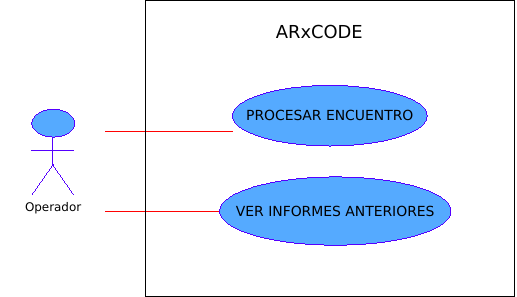
\includegraphics[width=.5\textwidth]{imagenes/usecaseAR}
  \caption{Casos de Uso de ARxCODE}
  \label{fig:casosuso}
\end{figure}


 \begin{table}[h]\renewcommand{\arraystretch}{1.3}
 \caption[Caso de Uso: Procesar Encuentro]{Caso de uso: \it{Procesar Encuentro}}
\centering
\resizebox{17cm}{!}{
\begin{tabular}[c]{ll}
\hline 
\rowcolor{lightgray}
\bf{Nombre}  &    {\it{\bf{Procesar Encuentro}}}\\
\hline
Actor  &    Operador de Din\'amica Orbital con Autorizaci\'on\\
\hline
\multirow{ 3}{*}{Prop\'osito} & Calcular la probabilidad de colisi\'on, la m\'inima distancia total\\
& y m\'inima distancia en la coordenada radial, para poder hacer un an\'alisis\\
& de la situaci\'on de encuentro.\\
\hline
\multirow{ 4}{*}{Resumen}& Procesa la ingesta de datos de un encuentro.\\
&  y calcula los par\'ametros de la situaci\'on de riesgo:\\
& m\'inima distancia total, m\'inima distancia en la coordenada radial y probabilidad de colisi\'on.\\
& Realiza gr\'aficos e informes.\\
\hline
\multirow{ 3}{*}{Precondiciones}  &  El operador debe estar registrado en la p\'agina space-track de NORAD.  \\
& Los archivos CDM deben estar previamente cargados en el Directorio de b\'usqueda.\\
& El operador debe conocer el encuentro que desea analizar y sus datos en caso del ingreso manual.\\
\hline
\multirow{ 3}{*}{Flujo Principal} & 1 - El operador selecciona un archivo con un mensaje de alerta. \\
& 2 - El operador oprime el bot\'on {\it{Track}} para visualizar el encuentro proyectado en la superficie terrestre (opcional)\\
& 3 - El operador oprime el bot\'on para generar un informe (opcional)\\
\hline
\multirow{ 3}{*}{Flujo Alternativo} & 1 - El operador ingresa los n\'umeros de identificaci\'on de los objetos (NORAD\_ID) \\
& 2 - El operador ingresa la fecha y hora del m\'aximo acercamiento (TCA)\\
& 3 - El operador oprime el bot\'on {\it{Procesar}} para procesar el encuentro\\
\hline
Postcondiciones & El informe de an\'alisis de riesgo fue generado y almacenado.\\
\hline
\end{tabular}}
\label{tab:usoproceso}
\end{table}

\subsection{Ámbito del sistema}
Se evalu\'o  el concepto del ARxCODE en el contexto de la Unidad de Desarrollo de Desechos Espaciales de la CONAE. Fundamentalmente la vinculaci\'on con el departamento de Din\'amica Orbital y los procedimientos actuales que se realizan en relaci\'on a los riesgos de colisi\'on con desechos.\\

Se hizo un estudio de las estructuras org\'anicas existentes y los sistemas asociados. Los distintos tipos de productos y usuarios, las interfaces que existen y el acceso a los datos reales con los que se  podr\'ia contar.\\

Se analiz\'o c\'omo trabajan otras agencias espaciales el problema de los desechos espaciales y se sacaron conclusiones respecto de qu\'e es lo que podr\'ia ofrecerse y bajo qu\'e premisas.\\

De las consideraciones m\'as importantes que se desprendieron de esta etapa, cabe destacar que se decidi\'o un prototipo para funcionar montado sobre el software principal de Din\'amica Orbital, como un anexo que no interfiere de ninguna manera con los procesos actuales. Así mismo, sus productos finales no ser\'an considerados en la toma de decisiones hasta tanto sus resultados no hayan sido validados durante un periodo suficiente, que permita verificar y mejorar su funcionamiento, contrast\'andolo con un acumulado de situaciones reales.\\

\subsection{Caracter\'isticas de los Usuarios}
Debido a la complejidad del problema y sus consecuencias, ser\'a un software diseñado para ser utilizado por un analista experto, con conocimientos de Din\'amica Orbital.\\

\subsection{Restricciones}
Se cont\'o con el asesoramiento y el intercambio de informaci\'on con personas del \'area de Din\'amica Orbital y otros departamentos de la CONAE. Se realizaron algunas reuniones e intercambio de correos electr\'onicos, aunque por ser una tem\'atica que se aborda bajo reg\'imenes especiales de acuerdos de confidencialidad, no fue posible contar con la totalidad de la informaci\'on.\\

\subsection{Interfaces}
ARxCODE fue pensado para ser un sistema anexo a las estructuras del departamento de Din\'amica Orbital. El dise\~no completo, contempla un acceso directo al servidor de la base de datos de los productos de Din\'amica Orbital para la obtenci\'on de: las efem\'erides propagadas de la misi\'on operativa, y los mensajes de alerta (CDM). Estos \'ultimos tambi\'en podr\'an ser recibidos por correos electr\'onicos de los organismos internacionales de alerta, como por ejemplo JSpOC o mediante una solicitud a la p\'agina Space-track, previa notificaci\'on y registro autorizado del operador a cargo, (Fig. \ref{fig:interfaces}).\\

\begin{figure}
\centering
  \fbox{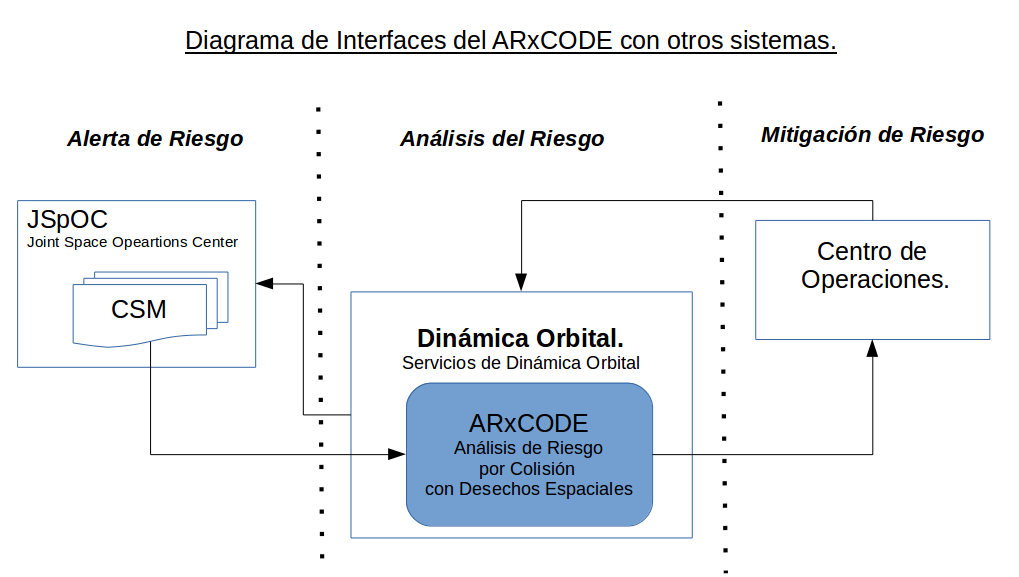
\includegraphics[width=0.8\textwidth]{imagenes/interfasessistemas}}
  \caption[Diagrama de Interfaces del Sistema]{Diagrama de Interfaces del Sistema}
  \label{fig:interfaces}
\end{figure}



\section{Especificaciones Finales}

\subsection{Requerimientos Finales}
El sistema debe tener la capacidad de interpretar los mensajes estandarizados CDM y presentar la informaci\'on que all\'i se registra, en forma clara al operador. Por otro lado, debe tener la capacidad de colectar datos ingresados manualmente por el operador y ofrecer los par\'ametros que resulten del procesamiento propio del ARxCODE, como m\'inima distancia, TCA calculado y PoC.\\

Esta \'ultima funcionalidad implica que ARxCODE debe poder solicitar a la p\'agina Space-Track los TLEs correspondientes a los objetos involucrados, debe poder estimar las matrices de covarianza de ambos objetos, ya sea mediante el m\'etodo de Osweiler o incorporando efem\'erides predichas del departamento de Din\'amica Orbital; debe poder propagar esos errores al momento del TCA y finalmente calcular la PoC.
En la Tabla \ref{tab:reqfinales}, se listan todos los requerimientos del sistema.\\

\begin{table}[!h]\renewcommand{\arraystretch}{1.3}
\caption[Tabla de Requerimientos]{Tabla de especificaci\'on de requerimientos del ARxCODE}
 \resizebox{\linewidth}{!}{
 \begin{tabular}{ll}
 \hline \hline 
   \rowcolor{lightgray}
  Req. ID & Descripci\'on \\
  \hline \hline
  \rowcolor{lightgray}
  1 & Requerimientos FUNCIONALES\\
  \hline 
  ARR-010 & ARxCODE debe calcular la probabilidad de colisi\'on de un acercamiento de riesgo.\\  
  \hline
  \multirow{2}{*}{ARR-020} & ARxCODE debe  aceptar como inputs: un mensaje de alerta (CDM), o los identificadores\\
  & de NORAD de ambos objetos y el tiempo de m\'aximo acercamiento (TCA).\\  
  \hline
  \multirow{2}{*}{ARR-030} & ARxCODE debe utilizar los productos orbitales de la misi\'on o realizar el mismo\\
  & procedimiento que se aplica al desecho, a la misi\'on.\\  
  \hline
  ARR-040 & ARxCODE debe calcular la m\'inima distancia, total y en la coordenada radial.\\ 
  \hline
  ARR-050 & ARxCODE debe manipular los sistemas de referencia: TEME, TOD y RTN. \\
  \hline
  \multirow{2}{*}{ARR-060}& ARxCODE debe permitir al operador analista experto visualizar el encuentro,\\
  & generar reportes y notificaciones.\\
  \hline
  \multirow{2}{*}{ARR-070} & ARxCODE debe extraer el conjunto de TLEs de los objetos involucrados \\
  & de los \'ultimos 15 d\'ias anteriores al TCA.\\
  \hline
  ARR-080 & ARxCODE debe estimar los errores en la posici\'on inicial del desecho y de la misi\'on operativa.\\
  \hline
  ARR-090 & ARxCODE debe propagar los errores de la posici\'on inicial al TCA.\\
  \hline
   \rowcolor{lightgray}
  2 & Requerimientos de INTERFACES \\
  \hline 
  ARR-100 & ARxCODE deber\'a permitir la carga manual de la situaci\'on de encuentro.\\
  \hline
  ARR-110 & ARxCODE deber\'a descargar los TLE de Space-Track.\\
  \hline
  ARR-120 & ARxCODE deber\'a manipular los CDM con formato xml.\\
  \hline
   \rowcolor{lightgray}
  3 & Requerimientos de RENDIMIENTO y/o PERFORMANCE\\
  \hline 
  ARR-210 & ARxCODE deber\'a ofrecer el reporte de la situaci\'on en no m\'as de 1 minuto. \\
  \hline
    \rowcolor{lightgray}
  4 & Requerimientos de VALIDACI\'ON \\
  \hline 
  \multirow{2}{*}{ARR-300} & Los m\'odulos de implementaci\'on de metodolog\'ias de ARxCODE ser\'an validados\\
  & con los resultados de las publicaciones pertinentes y de la bibliograf\'ia.\\
  \hline
  ARR-310 & Las propagaciones realizadas con el SGP4 ser\'an validadas con el software STK. \\
  \hline
    \rowcolor{lightgray}
  5 & Requerimientos de DISE\~NO\\
  \hline 
  ARR-400 & ARxCODE tendr\'a un dise\~no modular.\\
   \hline
  ARR-410 & ARxCODE se desarrollar\'a como una librer\'ia. \\
  \hline
  ARR-420 & ARxCODE contar\'a con una interfaz gr\'afica. \\
  \hline
    \rowcolor{lightgray}
  6 & Requerimientos de IMPLEMENTACI\'ON\\
  \hline 
  ARR-500& ARxCODE ser\'a implementado en python 2.7.\\
  \hline
  ARR-510& ARxCODE ser\'a implementado en el entorno de desarrollo Eclipse.\\
  \hline
  ARR-520& El control de versiones se realizar\'a con el gestor Git.\\
  \hline
    \rowcolor{lightgray}
  7 & Requerimientos de REUSABILIDAD\\
  \hline 
  ARR-600 & ARxCODE utilizar\'a la librer\'ia de SGP4 en Python. \\
  \hline
  ARR-610 & ARxCODE utilizar\'a la librer\'ia de Element Tree para el parseo del CDM.\\
  \hline
  ARR-620 & ARxCODE utilizar\'a la librer\'ia de requests de python para la conexi\'on con Space-Track.\\
  \hline
  ARR-630 & ARxCODE utilizar\'a la librer\'ia de numpy y scipy de python para los c\'alculos estad\'isticos y de integraci\'on. \\
  \hline
 \end{tabular}
 }
 \label{tab:reqfinales}
\end{table}


\section{Flujo din\'amico de ARxCODE}

ARxCODE se inicializa cuando un operador lo ejecuta. Una vez iniciado el programa, el operador debe seleccionar alguna de las dos opciones de procesamiento: {\it{Cargar CDM}} o {\it{Carga Manual}}. Una vez cargados los datos se inicia la etapa del PROCESAMIENTO.

\subsection*{Procesamiento a partir de un CDM}
Si el procesamiento se realiza a partir de la carga de un CDM, el c\'odigo se ocupa de la extracci\'on y la publicaci\'on de los datos del CDM. 
\subsection*{Procesamiento a partir de una carga manual}
En el caso de la carga manual, el procesamiento implica distintos pasos (Fig. \ref{fig:actdiag}):
\begin{itemize}
 \item Solicita los TLE a NORAD.
 \item Propaga los TLE y calcula el TCA y la m\'inima distancia.
 \item Calcula la covarianza del desecho, y de la misi\'on si la misma no fue provista por el departamento de Din\'amica Orbital.
 \item Calcula la matriz de covarianza combinada.
 \item Propaga la matriz de covarianza combinada hasta el TCA.
 \item Calcula la probabilidad de colisi\'on.
 \item Publica los datos en la pantalla para el operador.
\end{itemize}

Finalizada esta etapa de procesamiento y publicaci\'on de los datos por pantalla, el operador puede solicitar la visualizaci\'on de las trayectorias en el intervalo analizado, para ello presiona el bot\'on {\it{Track}} y el gr\'afico se agrega a la pantalla.\\

\begin{figure}[h!]
  \centering
  \fbox{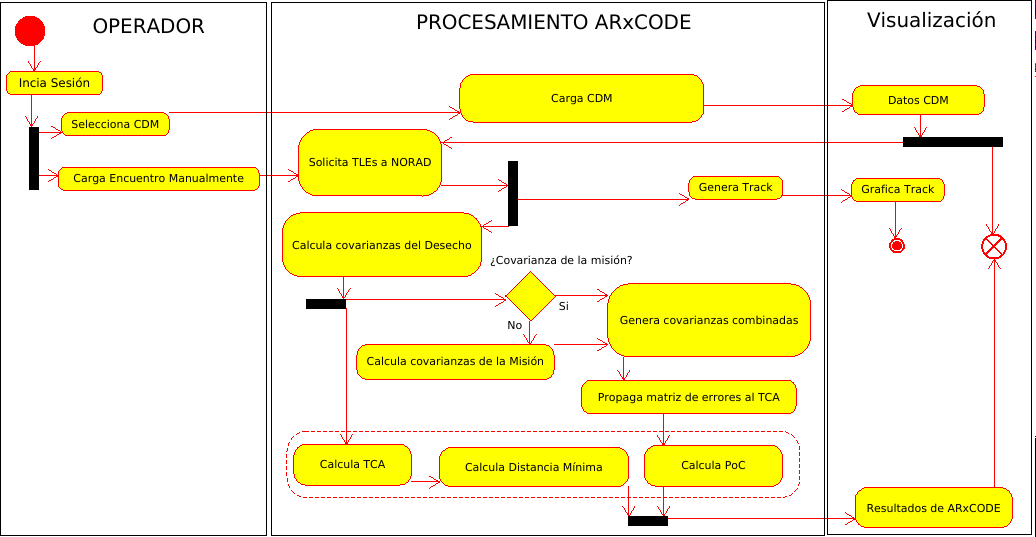
\includegraphics[width=\textwidth]{imagenes/actdiagAR}}
  \caption{Diagrama de Actividades de ARxCODE}
  \label{fig:actdiag}
\end{figure}

